\subsection{Анализ узкого места}

Была выдвинута гипотеза, заключающаяся в том что Dream EML показывает плохие результаты из-за большого количества аллокаций.
Дело в том что для сохранения чистоты функций, используемых dream eml, для каждого шаблона создается свой буфер для временных данных.
Проверить эту гипотезу несложно, достаточно запустить инструменты замера количества аллокаций. Результаты представлены в этой таблице:

% // TODO: добавить таблицу результатов запуска valgrind

Как видно, количество аллокаций растет линейно с размером программы.
Однако, эти аллокации не являются необходимыми и сразу же выкидываются после завершения исполнения функции.

Была предпринята попытка добавить пул из заранее аллоцированных буферов для рендеринга и заменить создание новых буферов на взятие их из пула.
EML является препроцессором и не добавляется в рантайм приложений как зависимость, поэтому добавить общий рантайм для всех файлов проходящих через препроцессинг не представляется возможным.
В связи с этим, этот пул создавается в начале каждого файла, проходящего через препроцессинг.

Для добавления такого пула был создан токен начала файла, который в последствии преобразуется в код создания пула.
Старый код создания локальных буферов был заменен на вызов функции получения буфера из пула.
Вместо вызова функции получения текста из буфера был добавлен код возврата буфера в пул с его последующим очищением.
Пул сделан параметризируемым по размеру буфера и количеству буферов создаваемых на момент инициализации программы.
Параметры принимаются как аргументы запуска препроцессора: --buffer-size и --pool-size.
Поскольку создать общий рантайм или библиотеку не представляется возможным, дабы не вызвать конфликт имен, все имена функций были префиксированы с тремя нижними подчеркиваниями.

\subsection{Механизм пула буферов}

OCaml\footnote{Dream EML также поддерживает синтаксис Reason, для которого была написана своя реализация. Поскольку суть не меняется, в работе она не приводится.} код пула буферов, вставляемый в начале каждого файла выглядит следующим образом:

\begin{lstlisting}
let ___eml_pool = ref (
    List.init ___EML_POOL_SIZE 
    (fun _ -> Buffer.create ___EML_BUFFER_SIZE)
)
let ___eml_get_buffer pool =
    match !pool with
    | buf :: bufs ->
        pool := bufs;
        Buffer.clear buf;
        buf
    | [] -> Buffer.create ___EML_BUFFER_SIZE
let ___eml_return_buffer pool buf =
    pool := buf :: !pool;
    Buffer.contents buf
\end{lstlisting}

Поскольку OCaml имеет кооперативную модель многопоточности, весь пул представляет собой простой связанный список.
Секвенциальное исполнение кода гарантирует что за раз пул будет отдаваться только одному потоку.
В счязи с этим чаще всего, для простых серверов достаточно будет иметь всего 1 буфер в этом пуле, который постоянно переиспользуется.
% // TODO https://sci-hub.ru/10.1145/3192366.3192421 - про модель памяти в ocaml
% // TODO попробовать сделать тест и на это?



\subsection{Результат оптимизации}

\begin{figure}[h!]
    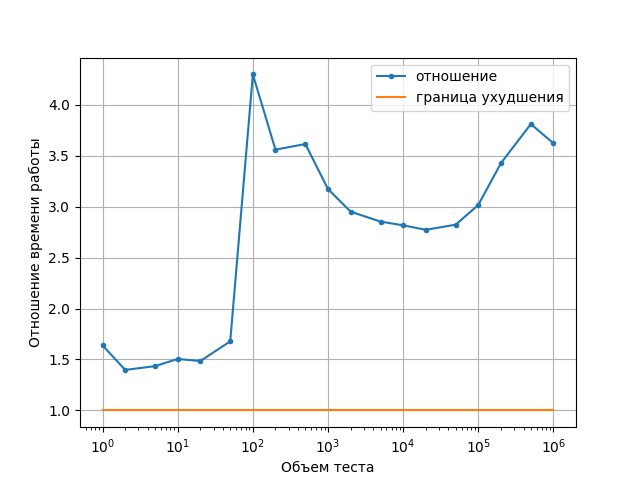
\includegraphics[width=\textwidth]{ratio.png}
    \caption{Результат оптимизации пула буферов. Построен с помощью matplotlib. Показано отношение времени работы до оптимизации к времени после. Граница ухудшения - значение отношения равное 1, что соответствует границе после которой считается что скорость увеличилась.}
    \label{fig:ratio}
\end{figure}

Как видно из сравнительного графика \ref{fig:ratio} в среднем производительность увеличилась в 2.65 раз.

\subsection{Дополнительный анализ}

По умолчанию создается всего 1 буфер размером 4096 символов.
Эти настройки не являются оптимальными для всех страниц, однако являются достаточно гибкими для большинства страниц.
Страницы, имеющие большой объем текста, могут создавать меньшее количество буферов с бОльшим размером.
% Эта настрйока релевантна для страниц, имеющих обратную проблему - малое количество рендерингов большого объема. % // TODO: сделать бенчмарк доказывающий это утверждение должно быть несложно

